\chapter{Symmetry, Energy, and the Hamiltonian}

After a long informal prelude, Leonard Susskind begins the formal lecture by going back. He says, in effect, that the previous discussion of symmetry and conservation laws left something blurred, and the blurred point is not a technicality. It is the meaning of symmetry itself, especially the distinction between active and passive transformations. Only after that point is repaired does the lecture turn to the missing conservation law, energy, and from there to the Hamiltonian. These notes follow that unfolding closely, with the preserved board figures kept as supporting lecture evidence; the note-writing curation is by LazyingArt LLC and Video2Book.

\section{Return to Symmetry and Active Transformations}

Susskind reopens the subject in repair mode: let us go back a little bit to what is at least half the heart of the subject, symmetries and conservation laws. The place to begin is a very simple instruction,
\[
x\to x+1,
\]
for a particle on a line. What exactly does that mean?

The lecture insists that the same formal rule can conceal two physically different operations. In the passive version we merely relabel the points of the line. The point formerly called \(x=0\) is now called \(x'=1\), but the particle has not moved at all. If there is a potential energy, it does not change, because the particle remains in the same place relative to the world.

In the active version we keep the labels fixed and move the particle itself. If it was at \(x\), we take it to \(x+1\). Now the potential energy may change, because the particle has moved relative to the environment that produced the potential.

This is the point Susskind wanted to sharpen. A particle moving in a potential is already a partial description of a larger system. We are tracking the particle while treating the Earth, or the apparatus, or some other heavy structure as fixed.

\subsection{Question \& Answer}

\paragraph{Question.} If the potential changes when the particle is shifted, does that mean the source of the potential is not being counted as part of the system?

\paragraph{Answer.} Exactly. The lecture makes this explicit. In treating a particle in a potential we have divided the world into two pieces: the particle, and everything else that generates the potential. If we shifted the entire system, including the Earth or the external source, the potential energy would not change. But that is not the approximation we are making. We are studying the motion of the particle relative to fixed external structure.

Once that is clear, Susskind passes from the example of a line to the general configuration space of coordinates \(q_i\). A configuration is a point in that space. An active infinitesimal transformation takes every point to a nearby point,
\begin{equation}
\delta q_i=\epsilon f_i(q).
\end{equation}
Here \(\epsilon\) is a small bookkeeping parameter. The functions \(f_i(q)\) are fixed once and for all by the transformation, but they may depend on where one is in configuration space. Some of them may vanish; that simply means some coordinates are not shifted.

The lecture also insists that the rule of transformation is time-independent. When we say \(x\to x+\epsilon\), we mean at all times. The same transformed history is used at \(t\), at \(t+\delta t\), and so on. For that reason the variation of a velocity is obtained by differentiating the variation of the coordinate:
\begin{equation}
\delta \dot q_i=\frac{d}{dt}\bigl(\delta q_i\bigr).
\end{equation}
For a pure translation,
\begin{equation}
x\to x+\epsilon,
\qquad
\delta \dot x=0,
\end{equation}
because the shift is a constant. But in a coordinate-dependent transformation, such as a rotation, the velocities do change.

\subsection{Question \& Answer}

\paragraph{Question.} If the transformation is time-independent, why did the rotation example change the velocities?

\paragraph{Answer.} Because the rule is time-independent, but the coordinate variation need not be a constant. The general rule is
\[
\delta \dot q_i=\frac{d}{dt}(\delta q_i).
\]
For a translation, \(\delta x=\epsilon\), so its time derivative vanishes. For a rotation, \(\delta x\) and \(\delta y\) depend on \(x\) and \(y\), so differentiating them produces terms involving \(\dot x\) and \(\dot y\). That is why the velocities rotate along with the positions.

\section{When Is a Transformation Really a Symmetry?}

Now comes the sharper question. Under an active transformation, the potential energy will generally change. The kinetic energy may change too. In non-Cartesian coordinates the kinetic term itself can depend on the coordinates; the familiar polar-coordinate term \(r^2\dot\theta^2\) is the simplest reminder. More generally, the Lagrangian may not divide neatly into a conventional kinetic part and a conventional potential part at all. It may simply be some function of \(q\), \(\dot q\), and perhaps \(t\).

So what does it mean to say that a transformation is a symmetry? Susskind answers in two steps.

First, it is the whole Lagrangian that matters. Second, the invariance must hold everywhere in configuration space, not merely at the particular point where the system happens to be.

Let us see this first in the simplest possible case. Suppose the potential energy is \(V(x,y)\), and we consider a small shift in the \(x\)-direction. Then
\begin{equation}
\delta V=\frac{\partial V}{\partial x}\,\delta x.
\end{equation}
If the potential does not change under the shift, and this is true no matter where the particle could be, then
\begin{equation}
\frac{\partial V}{\partial x}=0.
\end{equation}
Thus the potential is independent of \(x\). If the same statement held in every direction, the potential would be constant. This is precisely what the lecture means by saying that the potential energy is unchanged under translation.

The same logic applies to the Lagrangian. For an infinitesimal transformation, the strongest natural statement is that there is no first-order change. In compact reconstructed form we may write
\begin{equation}
\delta L = O(\epsilon^2),
\end{equation}
meaning that the variation has no term proportional to \(\epsilon\). The lecture states this verbally: no first-order change, no change proportional to the small parameter itself.

That is enough. If the first-order change vanishes at every point in configuration space, then repeating the infinitesimal transformation builds up a finite transformation that also leaves the Lagrangian unchanged.

There is also a modest mathematical assumption quietly built into the whole discussion: the functions are differentiable. The lecture briefly pauses over worries about cusps and direction-dependent derivatives and then sets them aside. For present purposes the functions are smooth enough that these variations make sense in the ordinary way.

\subsection{Question \& Answer}

\paragraph{Question.} Does symmetry require the kinetic and potential energies to remain unchanged separately? And when we say ``the Lagrangian does not change,'' do we mean exactly zero change or merely a negligibly small one?

\paragraph{Answer.} Only the whole Lagrangian matters. In many interesting cases one cannot even ask for separate invariance of kinetic and potential terms, because the Lagrangian does not split that way. And because the transformation is infinitesimal, ``no change'' means no first-order change. Terms of order \(\epsilon^2\) are not the issue; the symmetry condition is the absence of the linear term.

\section{Noether Charge, Translation, and Rotation}

Once the criterion for symmetry is fixed, the conserved quantity can be written down. Susskind does not rederive it here; he says that was done before. The result is that if
\[
\delta q_i=\epsilon f_i(q)
\]
is an ordinary symmetry, then there is a conserved quantity
\begin{equation}
Q=\sum_i p_i f_i(q),
\qquad
p_i=\frac{\partial L}{\partial \dot q_i},
\qquad
\dot Q=0.
\end{equation}
In speech he says that last time he called it \(q\) for ``quantity.'' In the notes it is clearer to denote it by \(Q\).

Let us first remind ourselves of translation symmetry. For a shift in the \(x\)-direction we have
\begin{equation}
\delta x=\epsilon,
\qquad
f_x=1.
\end{equation}
Then the conserved quantity is just the momentum in the \(x\)-direction:
\[
Q=p_x.
\]
If the system is fully translation invariant, then similarly \(p_y\) and \(p_z\) are conserved. If there are many particles, the symmetry is not the motion of one particle relative to the others; it is the simultaneous displacement of the whole system. In that case the conserved quantity is the total momentum, for example
\begin{equation}
P_x^{\mathrm{tot}}=\sum_a p_{x,a}.
\end{equation}

Rotation is slightly less trivial, and the lecture deliberately checks it geometrically. In the plane, an infinitesimal rigid rotation takes the form
\begin{equation}
\delta x=-y\,\epsilon,
\qquad
\delta y=x\,\epsilon.
\end{equation}
A quick check is to see whether the squared distance from the origin is preserved:
\begin{equation}
r^2=x^2+y^2.
\end{equation}
Its variation is
\begin{equation}
\delta(r^2)=2x\,\delta x+2y\,\delta y.
\end{equation}
Substituting the rotational shifts,
\begin{equation}
\delta(r^2)=2x(-y\,\epsilon)+2y(x\,\epsilon)=0.
\end{equation}
So the transformation is indeed a rigid infinitesimal rotation.

Because the coordinate shift depends on position, the velocities shift as well:
\begin{equation}
\delta \dot x=-\dot y\,\epsilon,
\qquad
\delta \dot y=\dot x\,\epsilon.
\end{equation}
Therefore \(\dot x^2+\dot y^2\) is unchanged, and if the potential depends only on radial distance, the full Lagrangian is invariant.

Now we feed the rotational \(f_i\) into the Noether formula. The conserved quantity is
\begin{equation}
Q=p_x(-y)+p_y(x)=-y\,p_x+x\,p_y.
\end{equation}
This is the \(z\)-component of angular momentum,
\begin{equation}
Q=(\mathbf r\times \mathbf p)_z.
\end{equation}
In three dimensions one gets the other components by rotating the other coordinate planes. For many particles, if the whole system is rotationally invariant, then the conserved quantity is the total angular momentum,
\begin{equation}
\mathbf L_{\mathrm{tot}}=\sum_a \mathbf r_a\times \mathbf p_a.
\end{equation}

By this point the lecture has accounted for momentum conservation and angular momentum conservation. That makes the missing case conspicuous: what about energy?

\section{Time Translation Invariance and Explicit Time Dependence}

Now we come to the real question of the lecture. Is energy conservation also associated with a symmetry?

\subsection{Question \& Answer}

\paragraph{Question.} Is energy conservation another Noether theorem, and if so, what symmetry is responsible for it?

\paragraph{Answer.} Yes. But it is not an ordinary symmetry of the \(q_i\). It is time translation invariance.

Susskind introduces this operationally. Imagine an experiment that begins at time \(t_0\), ends at time \(t_1\), and yields some result. Now shift the entire experiment later by \(\delta t\): start later, end later, keep the same initial conditions, and ask whether the outcome is unchanged. If it is, then the system is invariant under time translation.

The lecture is careful here, just as it was careful about the system-environment split earlier. A subsystem may fail to be time-translation invariant because some external agent is changing a parameter in time.

The first example is a charged particle between capacitor plates. If the capacitor is already charged and stays that way, shifting the experiment in time changes nothing. But if the plates are being charged up by an external battery or generator, then the result depends on when the particle is introduced. The particle alone is not a time-translation-invariant system.

The second example is the harmonic oscillator with a time-dependent spring constant:
\begin{equation}
L=\frac12 m\dot x^2-\frac12 k(t)x^2.
\end{equation}
If \(k\) varies with time, then knowing \(x\) and \(\dot x\) is not enough to know \(L\); one must also know the time. This is what the lecture means by explicit time dependence.

So the criterion is very simple:
\begin{equation}
\frac{\partial L}{\partial t}=0
\end{equation}
means that there is no explicit time dependence. This does not mean that \(L\) is constant along the actual motion. The coordinates and velocities are changing, so the numerical value of \(L\) may change as the system moves. It means only that there is no additional dependence on time beyond the dependence carried by \(q(t)\) and \(\dot q(t)\).

Susskind phrases it very concretely: if you know the \(q\)'s and the \(\dot q\)'s at an instant, do you already know the Lagrangian, or do you also have to know what time it is? If the answer is that \(q\) and \(\dot q\) suffice, then the system is time-translation invariant.

From the narrow point of view, time dependence in a parameter means no symmetry and no conservation of the subsystem's energy. From the larger point of view, where we include the external charging mechanism or the external device changing the spring constant, the full system does have time-translation invariance, and the full energy is conserved. The lecture returns to this theme repeatedly: non-conservation in the reduced description is really exchange with degrees of freedom we have chosen not to follow.

\section{From the Time Derivative of \(L\) to the Hamiltonian}

At this point the lecture makes a pedagogical feint. Suppose, Susskind says, that we did not already know the ordinary formula \(E=T+V\). Suppose we guessed that maybe the Lagrangian itself was the conserved energy. How would we test that guess? We would differentiate the Lagrangian with respect to time and see whether it is conserved.

\begin{figure}[htbp]
\centering

\includegraphics[width=0.62\textwidth]{lecture_05_figure_02.png}
\caption{Beginning the time-derivative calculation for the Lagrangian.}
\end{figure}

Along the actual trajectory of the system,
\begin{equation}
\frac{d}{dt}L(q_i,\dot q_i,t)
\end{equation}
is the total time derivative. By the chain rule,
\begin{equation}
\frac{dL}{dt}
=
\sum_i \frac{\partial L}{\partial q_i}\dot q_i
+
\sum_i \frac{\partial L}{\partial \dot q_i}\ddot q_i
+
\frac{\partial L}{\partial t}.
\end{equation}
The lecture first motivates this as basic calculus: differentiate with respect to each argument, then multiply by the time derivative of that argument. The sum over \(i\) is important; every coordinate contributes.

Now comes the small bit of magic, as he calls it. We use the canonical momentum definition
\begin{equation}
p_i=\frac{\partial L}{\partial \dot q_i},
\end{equation}
and the Euler--Lagrange equations in the form
\begin{equation}
\dot p_i=\frac{\partial L}{\partial q_i}.
\end{equation}
Substituting these into the chain rule gives
\begin{equation}
\frac{dL}{dt}
=
\sum_i \left(\dot p_i\dot q_i+p_i\ddot q_i\right)
+
\frac{\partial L}{\partial t}.
\end{equation}
But the expression in parentheses is just the derivative of a product:
\begin{equation}
\sum_i \left(\dot p_i\dot q_i+p_i\ddot q_i\right)
=
\frac{d}{dt}\sum_i p_i\dot q_i.
\end{equation}
Therefore
\begin{equation}
\frac{d}{dt}\left(L-\sum_i p_i\dot q_i\right)
=
\frac{\partial L}{\partial t}.
\end{equation}
The quantity in parentheses is the negative of what is historically called the Hamiltonian. So we define
\begin{equation}
H=\sum_i p_i\dot q_i-L,
\end{equation}
and obtain the general theorem
\begin{equation}
\frac{dH}{dt}=-\frac{\partial L}{\partial t}.
\end{equation}

\begin{figure}[htbp]
\centering

\includegraphics[width=0.55\textwidth]{lecture_05_figure_04.png}
\caption{Hamiltonian change from explicit time dependence of the Lagrangian.}
\end{figure}

This is the payoff. If there is no explicit time dependence, \(\partial L/\partial t=0\), then
\begin{equation}
\dot H=0.
\end{equation}
So time translation invariance gives a conserved quantity, and that conserved quantity is the Hamiltonian.

For the standard one-particle example,
\begin{equation}
L=\frac12 m\dot x^2-V(x),
\end{equation}
we have
\begin{equation}
p=\frac{\partial L}{\partial \dot x}=m\dot x.
\end{equation}
Hence
\begin{align}
H&=p\dot x-L \\
&=m\dot x^2-\left(\frac12 m\dot x^2-V(x)\right) \\
&=\frac12 m\dot x^2+V(x).
\end{align}
So in the familiar separable case the Hamiltonian is exactly the ordinary energy,
\begin{equation}
H=T+V.
\end{equation}

The time-dependent oscillator shows the general theorem at work. If
\begin{equation}
L=\frac12 m\dot x^2-\frac12 k(t)x^2,
\end{equation}
then holding \(x\) and \(\dot x\) fixed while differentiating only the explicit time dependence gives
\begin{equation}
\frac{\partial L}{\partial t}=-\frac12 \dot k(t)x^2.
\end{equation}
Therefore
\begin{equation}
\dot H=\frac12 \dot k(t)x^2.
\end{equation}
The energy of the oscillator is not conserved, because the external agent changing \(k(t)\) is pumping energy into or out of it. Again, the subsystem exchanges energy with the part of the world we have chosen not to include.

The lecture makes one more point explicitly: the Hamiltonian is the definition of energy, period. In familiar cases it reduces to kinetic plus potential, but that is a special recognition, not the general definition.

\section{Board Recap and Why the Lagrangian is Useful}

After the derivation, Susskind stops and does exactly what a good lecturer does after a long calculation: he summarizes everything on the board in one compact stack.

\begin{figure}[htbp]
\centering

\includegraphics[width=0.58\textwidth]{lecture_05_figure_03.png}
\caption{Lagrangian, canonical momentum, and the start of the Euler--Lagrange equation.}
\end{figure}

In cleaned form, the recap is
\begin{align}
L&=L(q_i,\dot q_i,t), \\
p_i&=\frac{\partial L}{\partial \dot q_i}, \\
\dot p_i&=\frac{\partial L}{\partial q_i}, \\
Q&=\sum_i p_i f_i(q), \qquad \dot Q=0, \\
H&=\sum_i p_i\dot q_i-L, \\
\dot H&=-\frac{\partial L}{\partial t}.
\end{align}
The board shows the top two lines clearly and only the beginning of the lower \(\dot p\) line; the completed form \(\dot p_i=\partial L/\partial q_i\) is the standard completion supported by the spoken recap.

This is the moment in the lecture when the formalism stops looking like a pile of separate tricks and begins to look like a small, coherent machine. One defines \(p_i\), writes the equations of motion, identifies Noether charges for ordinary symmetries, and identifies the Hamiltonian for time translation.

The lecture then shifts from foundations to utility. Why should one actually use the Lagrangian method? The answer is not that it is philosophically grander than \(F=ma\). The answer is that it is often easier.

Susskind's example is the double pendulum. If one attacks it directly with forces, one must keep track of constraints, tensions, and moving reference directions. The Lagrangian method begins more naturally: choose coordinates adapted to the motion, compute the kinetic and potential energies in those coordinates, and then let the Euler--Lagrange equations do the rest.

\begin{figure}[htbp]
\centering

\includegraphics[width=0.82\textwidth]{lecture_05_figure_05.png}
\caption{Hamiltonian time dependence beside a double-pendulum sketch.}
\end{figure}

A cleaned schematic of the board sketch is useful here:

\begin{figure}[htbp]
\centering
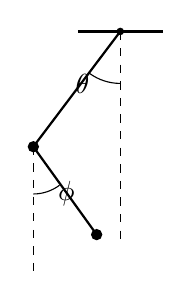
\begin{tikzpicture}[scale=1.2]
\draw[thick] (-0.45,0) -- (0.45,0);
\fill (0,0) circle (0.04);
\draw[dashed] (0,0) -- (0,-2.25);
\draw[thick] (0,0) -- (-0.92,-1.22);
\fill (-0.92,-1.22) circle (0.06);
\draw[dashed] (-0.92,-1.22) -- (-0.92,-2.55);
\draw[thick] (-0.92,-1.22) -- (-0.25,-2.15);
\fill (-0.25,-2.15) circle (0.06);
\draw (0,-0.55) arc (-90:-126:0.55);
\node at (-0.40,-0.55) {$\theta$};
\draw (-0.92,-1.72) arc (-90:-53:0.46);
\node at (-0.57,-1.72) {$\phi$};
\end{tikzpicture}
\caption{A cleaned double-pendulum schematic reconstructed from the board sketch.}
\end{figure}

The lecture does not carry out the full algebra, but it tells us how the calculation would go. Choose angular variables, perhaps \(\theta\) for the upper rod and \(\phi\) for the lower; compute the velocities of both masses in terms of those angles and their time derivatives; form \(T-V\); then derive the equations of motion. This is precisely the sort of problem for which the Lagrangian is a compact and powerful organizer.

The same point applies to change of variables more generally. If one wants to pass to a new coordinate system, it is often much easier to transform the Lagrangian and then rederive the equations than to transform the equations of motion one by one. The lecture notes, however, that time-dependent changes of variables, such as a rotating frame, are a separate beast; they are not the same as the fixed symmetries discussed earlier.

At this point Susskind also answers a natural structural question. Are the Lagrangian and Hamiltonian formulations two different theories of mechanics? No. They are equivalent. But they emphasize different aspects. The Lagrangian formulation emphasizes stationary action. The Hamiltonian formulation is more abstract and, historically, turned out to be central to quantum mechanics. The Hamiltonian is not merely the energy; it is the entrance to another way of organizing mechanics.

\section{A Nonstandard Lagrangian and the Limits of the Formalism}

To loosen the reader's dependence on the familiar \(T-V\) form, the lecture ends with a deliberately nonstandard example. From the Lagrangian point of view, there is nothing wrong with writing
\begin{equation}
L=\frac12 q^2\dot q^2-\frac12 q^2.
\end{equation}
Susskind remarks that one could add something like \(q\dot q\) as well, but he does not work that out; the explicit example on the board is the one above.

The canonical momentum is
\begin{equation}
p=\frac{\partial L}{\partial \dot q}=q^2\dot q.
\end{equation}
Differentiating with respect to time gives
\begin{equation}
\dot p=q^2\ddot q+2q\dot q^2.
\end{equation}
Meanwhile
\begin{equation}
\frac{\partial L}{\partial q}=q\dot q^2-q.
\end{equation}
So the Euler--Lagrange equation becomes
\begin{equation}
q^2\ddot q+2q\dot q^2=q\dot q^2-q,
\end{equation}
or, after simplifying,
\begin{equation}
q^2\ddot q+q\dot q^2=-q.
\end{equation}

\begin{figure}[htbp]
\centering

\includegraphics[width=0.78\textwidth]{lecture_05_figure_06.png}
\caption{Intermediate Euler--Lagrange algebra for the nonstandard Lagrangian example.}
\end{figure}

The board frame preserves the left-hand side of the intermediate step,
\[
q^2\ddot q+2q\dot q^2=,
\]
while the right-hand side is completed from the spoken derivation. This is a good example of how the screenshot and the transcript cooperate: the board preserves the working rhythm, the transcript supplies the missing completion.

The Hamiltonian is computed in the usual way:
\begin{equation}
H=p\dot q-L.
\end{equation}
Substituting \(p=q^2\dot q\),
\begin{align}
H&=q^2\dot q^2-\left(\frac12 q^2\dot q^2-\frac12 q^2\right) \\
&=\frac12 q^2\dot q^2+\frac12 q^2.
\end{align}
In this example the result again looks like a sum of two positive terms, so one may if one likes call them kinetic and potential pieces. But that is not the real lesson. The real lesson is that the formalism did not require us to begin from the conventional \(T-V\) split in order to derive equations of motion and define energy.

The final minutes of the lecture widen the scope. What about friction? Susskind's answer is blunt: ordinary finite-degree-of-freedom Lagrangian mechanics does not describe friction directly. Friction is not a primitive force at the level of elementary particles. It is a statistical effect of many microscopic degrees of freedom that we are not keeping track of. The same is true of inelastic collisions once one insists on following heat, internal excitation, and all the microscopic motion that carries the energy away.

This leads to the lecture's deepest closing remark. Why does classical mechanics take this Lagrangian and Hamiltonian form at all? One answer is experimental: real systems do. Another is constructive: one can guess a Lagrangian from symmetry or work backwards from equations of motion. But the deeper explanation, Susskind insists, lies in quantum mechanics. Classical mechanics does not precede quantum mechanics logically; quantum mechanics precedes classical mechanics logically. In quantum theory the Hamiltonian is the more primitive object, and classical mechanics inherits its very structure from that deeper framework.

\section{Summary}

Lecture~5 proceeds in a deliberate sequence. First it repairs the concept of symmetry by distinguishing passive relabeling from active motion relative to fixed external structure. Next it sharpens the symmetry criterion: the Lagrangian must have no first-order change, and this must hold everywhere in configuration space. Then it recalls the Noether charges for translation and rotation, making momentum and angular momentum conservation into direct consequences of symmetry.

Only after that does the lecture ask the missing question about energy. The answer is that energy comes from time translation invariance, and the conserved quantity is not the Lagrangian but
\[
H=\sum_i p_i\dot q_i-L.
\]
In the ordinary case \(H=T+V\), but the definition is much more general than that familiar form.

The closing examples widen the reader's sense of what the formalism is for. The Lagrangian is a powerful practical tool for choosing good coordinates and setting up difficult systems such as the double pendulum. It also makes sense beyond the simplest \(T-V\) models. But its limits are equally instructive: friction and dissipation point toward hidden degrees of freedom, and the deeper reason classical mechanics has this structure at all points beyond classical mechanics to quantum theory.